
% \section{Introduction}
% DEMOCRACY has problems and bureaucratic solutions
Democracies face two big problems. First, they are vulnerable to fleeting passions and demagogues. To combat this, they leave many decisions to experts who, ideally, %use wisdom and
exercises judgment loosely guided by the public. Second, everyone cannot vote on every decision. Thus, they delegate power to representatives (who then delegate it to deputies), create temporary mini-publics,
and solicit input from those most affected or moved by a public decision.\footnote{
As imagined by \citet{Dahl1989}, mini-publics are representative, selected at random, and deliberative. Besides juries, however, deliberative and randomly-selected bodies are rare. Instead, citizens more often engage in government decisions when given opportunities to opt-in, such as hearings, petitions, and public comment periods. These mechanisms of engagement generate a different, more contentious flavor of public input than the discourse imagined by scholars who focus on deliberation.
}
Most policy is then made by bureaucrats, supposedly guided indirectly through elected representatives and directly by limited public input (mostly limited to highly contentious policy debates).
By one estimate upward of 90\% of legally binding U.S. federal policy is now written by agencies \citep{West2013}.

% Both of these problems converge in the bureaucracy, run by experts who are deputized by elected officials (or by their deputy's deputy's deputy) and with procedures that create opportunities for public input. It is far from clear how bureaucratic decisions are to balance expertise, accountability to elected officials, and responsiveness to public input in decisionmaking. 


% \subsection{Why study rulemaking?}
% \section{The Importance of Studying Rulemaking}
% Mobilization may increasingly target rulemaking because it is how most policy in the U.S. is now made. 

% rulemaking matters 
With the rise of the administrative state, U.S. federal bureaucracy has become a major site of policymaking and political conflict. Agency rules are revised much more frequently than statutory law \citep{Wagner2017} and in the years or decades between legislative enactments, federal agencies make legally-binding rules interpreting and reinterpreting old statutes to address emerging issues and priorities. %Ninety percent of new policy that carries the force of law is now made in the bureaucracy rather than in Congress \citep{West2013}.\footnote{I use policy, law, and regulation as nested concepts. My methods generally apply to all policy texts whether they carry the force of law or not. Many public and private organizations, including agencies, have policy statements that are not legally binding. My empirical subject is rules that do carry the force of law based on some authorizing legislation. I use rule (a more technical term) and regulation (a more colloquial term) interchangeably.}
Examples are striking: The effect of the Dodd-Frank Wall Street Reform and Consumer Protection Act was largely unknown until the specific regulations were written, and it continues to change as these rules are revised. 
Congress authorizes billions in farm subsidies and leases for public lands, but who gets them depends on agency policy. In the decades since the last major environmental legislation, agencies have written thousands of pages of new environmental regulations and thousands more changing tack under each new administration. These revisions significantly shape lives and fortunes. For example, in 2006, citing the authority of statutes last amended in the 1950s, the Justice Department's Bureau of Prisons proposed a rule restricting eligibility for parole. In 2016, the Bureau withdrew this rule and announced it would be requiring fewer contracts with private prison companies, precipitating a 50\% loss of industry stock value. Six months later, a new attorney general announced these policies would again be reversed, leading to a 130\% increase in industry stock value. %Like many rulemaking debates, industry and advocacy groups spent millions of dollars lobbying on this issue. Few rulemakings, however, receive this level of public and presidential attention. In the majority of rulemakings, few participate, and we do not really know the extent to which participants get what they lobby for.% (but see Yackee and Yackee 2006)
Rulemaking clearly matters.

% democracy interbranch relations and autonomy
Less clear, however, is how the new centrality of agency rulemaking fits into American democracy. In addition the bureaucracy's complex relationships with the president and Congress, agencies have complex and poorly understood relationships with the public and advocacy groups. Relationships with constituent groups may even provide agencies with a degree of ``autonomy'' from their official principals \citep{Carpenter2001}. 

% 
Expertise, delegation, and limited public input converge in bureaucratic policymaking, where bureaucrats are required to use reasoned judgment, be accountable to elected officials, and be responsive to public input. There is no normative consensus on how to rank or merge these aims \citep{Wilson1967}, and administrative procedures for gathering public input and their justifications cite all three. Processes like notice and comment rulemaking are said to produce valuable technical information \citep{Yackee2006JPART, Nelson2012}, oversight opportunities \citep{Balla1998}, and democratic legitimacy \citep{Croley2003, Rosenbloom2003}. The Administrative Conference of the United States (ACUS) Proposed Recommendation on Public Engagement in Rulemaking claims that ``The opportunity for public engagement is vital to the rulemaking process, permitting agencies to obtain more comprehensive information, enhance the legitimacy and accountability of their decisions, and enhance public support for their rules'' \citep{ACUS2018}. 

% gap
Yet, legitimacy, accountability, public support, and especially collecting information depend not just on the opportunity to engage but actual engagement \citep{Herz2018}, and we know surprisingly little about the input of ordinary people and the role it may or may not play in rulemaking.\footnote{ 
But see \citet{Yackee2015JPART}, who surveys commenters, finding that members of the public believe their comments matter, even though powerful groups have more influence; \citet{Cuellar2005}, who examines three rules, finding that ordinary people made up the majority of commenters; and \citet{Balla2018}, who find significant participation from ordinary people in a case study of EPA rulemaking.} 


% \subsection{Models of Bureaucratic Politics} 
% MODELS HAVE NO PLACE 
The contentious politics that inspire ordinary people to engage have no place in leading models of bureaucratic policymaking and have largely been ignored by political scientists.
Instead, models focus on how agencies either learn about policy problems, negotiate or avoid accountability to various principals, or balance interest-group demands.\footnote{
On learning, see \citet{yackee2012} and \citet{Libgober2018} for an information-based model where commenting reveals information to the agency. 

On accountability to elected officials, see  \citet{Furlong1997}, \citet{Nou2016}, \citet{Potter2016}, \citet{Woods2018}, and \citet{Yackee2009RegGov}. For example, \citet{Potter2014dis} presents a signaling model where agencies propose and principals veto rules depending, in part, on their beliefs about interest group preferences. 

On interest group balancing see \citet{Yackee2006JOP},  \citet{Yackee2006JPART}, and \citet{Kerwin2011}.
} 
% SOPHISTICATED LOBBYING
% Influence in rulemaking is sophisticated lobbying efforts of powerful interest groups, whose role in shaping policy has been theoretically developed and empirically tested.

Foundational scholarship on rulemaking by \citet{Furlong2004}, \citet{Furlong1997, Furlong1998}, and \citet{Kerwin2011} focuses on interest group lobbying. To the extent they address it at all, both theory and empirical scholarship suggest skepticism that the input of ordinary people matters. 
% REREAD BERRY
% \citet{Berry1999TheGroups} argues that mass engagement occurs too late in the policy process to be effective compared to insiders who are able to shape agendas and alternatives. 
Empirical scholarship finds that economic elites and business groups dominate American politics in general \citep{Gilens2014} and rulemaking in particular \citep{Crow2015, Wagner2011, West2009, Yackee2006JOP, Yackee2006JPART, Yackee2012, Golden1998, Haeder2015}. %Perhaps this is unsurprising. 
% gap - REPRESENTATION - don't know who is represented
While some suggest that requirements for agencies to solicit and respond to public comments on proposed rules allow ``civil society'' to provide public oversight \citep{Michaels2015, Metzger2010}, others find that participants in rulemaking often represent elites \citep{Seifter2016UCLA} and business interests \citep{Yackee2006JOP}.
From a strategic perspective, agency officials are not directly accountable to voters. And even if organized groups do supplement congressional and judicial checks on executive power, the groups that participate in rulemaking represent only certain (if any) citizens and may not represent them well \citep{Seifter2016UCLA}. 
% From a science-based policy perspective, average citizens signing form letters provide no new information to policymakers. 
Mass comment campaigns are thus dismissed as epiphenomenal to bargaining with principals or interest groups. Indeed almost all empirical studies discard unsophisticated comments from ordinary people--i.e. not professional policy influencers.
Despite the skepticism assumed by scholars, \citet{Yackee2015JPART} finds that ordinary participants strongly believe that their comments matter, even if they see businesses as more influential.
Without systematic understanding and study of public participation, it is difficult to adjudicate debates about how processes like notice and comment rulemaking may enhance or undermine various democratic ideals.

% but so many mass comments
This scholarly oversight is surprising given that most people are only aware of rulemaking when it is the target of a high-profile mass mobilization campaign.\footnote{Some of the most contentious recent public controversies involve bureaucratic policymaking. For example, along with 50 thousand protesters in Washington D.C., the State Department Received 1.2 million comments on the Environmental Impact Statement for the Keystone Pipeline. Similarly, along with the thousands of protesters supporting the Standing Rock Sioux protest to the Dakota Access Pipeline, the Army Corps of Engineers received hundreds of thousands of comments. Alongside protest actions that included shutting down many websites, the Federal Communications Commission's open internet rule received 22 million comments. While some of these comments appear to be fake, the scale of public engagement is remarkable given how little attention political scientists have paid to it. Fake public comments also raise the question of why an organization would bother to generate fake public input if it did not matter, as its omission from theories of bureaucratic policymaking would seem to imply. %On each of these issues, advocacy activity has been followed by legislative or executive action.
} 
While most rules receive little attention, the ease of online mobilizing and commenting has, like other forms of participation \citep{Boulianne2018}, created exponential increases in the number of rules in which thousands and even millions of people engage (see figure \ref{fig:comments}; note that comments per rule are on a logarithmic scale).\footnote{Proposed rules that have attracted the most public attention have been published by the Federal Communications Commission (FCC, omitted from this plot), the Environmental Protection Agency (EPA), the Department of Interior (DOI), the Bureau of Ocean Energy Management (BOEM), the Consumer Financial Protection Bureau (CFPB), and Fish and Wildlife Service (FWS).} Occasionally, a large number of people are paying attention.

% adverse it as democracy 
The general failure to explain or account for mass engagement in rulemaking is also striking in light of how agencies advertise public comment periods as an opportunity for a voice in government decisions.\footnote{
% FOCUS
I focus on public comments in rulemaking, but my theory and methods also apply to other kinds of political engagement such as through social media or protests as well as to other political decisions, including state-level rulemaking. Social media engagement may be especially important if agencies implement the recommendations of \citet{ACUS2018} that ``Agencies should consider using social media before or in connection with direct final rulemaking to quickly identify whether there are significant or meaningful objections'' (p. 34). 
} 
Big red letters across the top of the Regulations.gov homepage solicit visitors to ``Make a difference. Submit your comments and let your voice be heard'' (Figure \ref{fig:regs.gov}). A blue "Comment Now!" button accompanies a short description of each draft policy and pending agency action. 
Another invitation at the bottom of the page reads ``Participate today!''
Public commenting on proposed agency rules is described as ``an important part of democracy'' (WSJ 2017), the ``purest example of participatory democracy in actual American governance'' \citep{Herz2016}. \citet{Rossi1997} finds that ``courts, Congress, and scholars have elevated participation [in rulemaking] to a sacrosanct status...greater participation is generally viewed as contributing to the democracy.'' % Is it?
Yet despite much debate about the theoretical import and possible reforms, the bulk of public comments have yet to be studied.

\begin{figure}[]
    \centering
    \caption{Regulations.gov Solicits Public Comments on Draft Agency Rules}
    \label{fig:regs.gov}
    
    
\includegraphics[width= 6.5in]{regulations-header.png}
\end{figure}

\begin{figure}
\caption{Comments on Proposed Rules per Year (left) and per Rule (right) posted on regulations.gov}
\centering
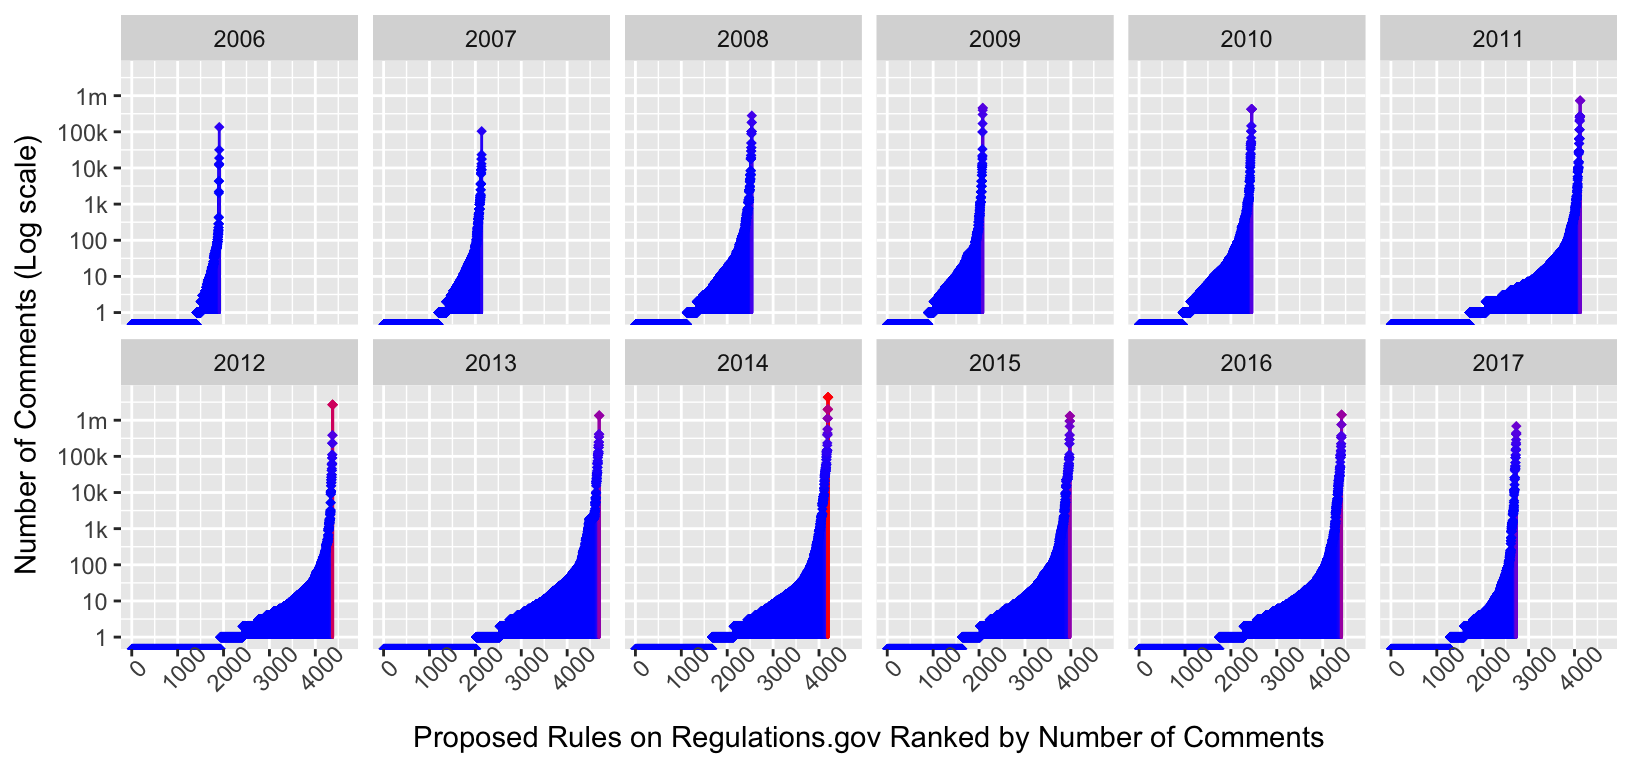
\includegraphics[height= 2.5in]{Figs/comments-per-year-1.png}
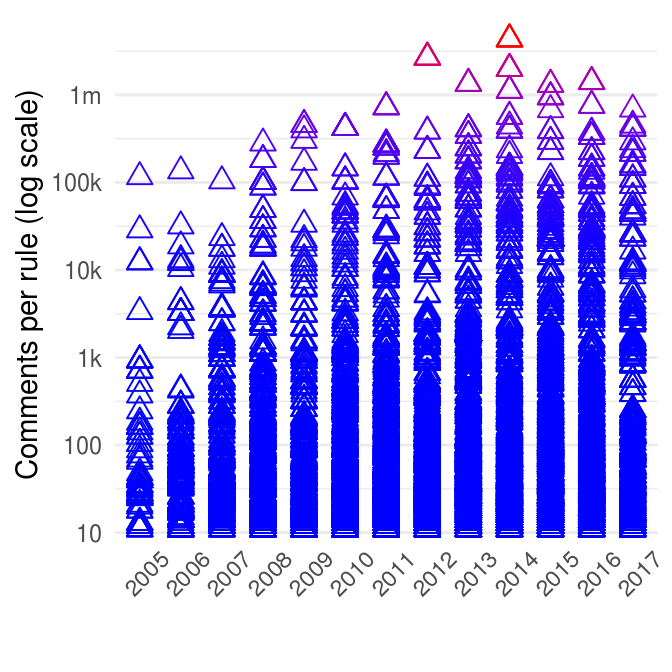
\includegraphics[height= 2.5in]{Figs/rules-comments-per-year-1.png}
\label{fig:comments}
\end{figure}

%It is even less clear whether actions by average citizens make a difference in agency policymaking. Many may believe that they do, but the mechanisms are not obvious. Indeed letter writing and other forms of mass mobilization do not have a clear place in political scientists' theories of bureaucratic politics. This lack of scholarship may be the result of both a general suspicion, rooted in certain theories of strategic behavior, that mass politics affects unelected career officials as well as a normative assumption that policy ``implementation'' is no place for contentious politics. Neither the bureaucrat who asserts that rules are the result of scientific analysis nor the political scientist who asserts that rules are the result of bureaucrats strategically selecting their most preferred policy within institutional constraints offer an explanation for why an agency would receive millions of public comments or why they would matter.











% LEGAL SCHOLARS' DEBATES 
Legal scholars have long debated what to make of mass commenting in rulemaking. Many focus on reforms to help agencies collect more useful information \citep{Farina2011, Farina2014, Rauch2016}. In 2018, ``Public engagement'' was main project of the Administrative Conference of the United States (ACUS) committee on Rulemaking: %\href{https://www.acus.gov/research-projects/public-engagement-rulemaking}
{The project} 
\begin{quote}``explores agency strategies to enhance public engagement prior to and during informal rulemaking. It seeks to ensure that agencies invest resources in a way that maximizes the probability that rulewriters obtain high-quality public information.'' 
\end{quote} 
Among other things, this committee is debating how to encourage ``quality public information,'' how ``to get new people/groups into the real or virtual room'' \citep{Farina2018}, and whether broad engagement is even desirable on all rules \citep{White2018}. Administrative law scholars have explored these questions for decades. \citet{Mendelson2011} finds that agencies often discard non-technical comments but argues that they should be given more weight. Others worry that mass commenting distracts agencies from good policy and the broader public interest \citep{Coglianese2006}. \citet[p. 112]{Farina2012} argues that ``[Mass] comments typically are neither factually informative nor reliable indicators of citizens’ informed value preferences.'' \citet{Rossi1997} argues that public comment processes should be largely eliminated. \citet[p. 208]{Herz2016} concludes ``The goal of e-rulemaking is to more fully capture such credible, specific, and relevant information, not to solicit the views of random, self-nominating members of the public.'' Early optimism among legal scholars that the internet would ``change everything'' \citep{Johnson1998} and that ``cyberdemocracy''  would enable more deliberative rulemaking has faded.  
While commenting and encouraging others to comment has become easier, \citet{Coglianese2006} finds that little else has changed. 
Here, the prediction that the internet would merely facilitate engagement among the like-minded \citep{Sunstein2001} has largely been correct.
Mass comment campaigns are thus often called ``spam'' \citep{Balla2018}.
In this prevailing view, ``high-quality'' and ``relevant'' mean novel technical information, not opinions.
Even scholars suggesting reforms aimed at ``regulatory democracy'' aim to increase the ``sophistication'' of ordinary peoples' comments \citep{Cuellar2014}. Notably, the ACUS draft recommendations on ``Mass and Fake Comments in Agency Rulemaking'' suggests that ``effective comments'' give ``reasons rather than just reactions'' \citep[p. 33]{ACUS2018}. If true, public reactions to proposed rules such as mass comments would have no effect in rulemaking. 

While this scholarship has improved the theory and practice of policy learning in rulemaking, focusing on sophisticated deliberation and technical information overlooks the potential role of political information.\footnote{but see insights from \citet{Golden1998}, \citet{Nelson2012}, and \citet{Rauch2016} on political information and \citet{Reich1966} and \citet{Seifter2016UCLA} on representation reviewed below.}











%%%%%%%%%%%%%%%%%%%%%%%%%%%%%%%%%%%%%







% MODEL - regulator is uncertain about backlash 
% org may reveal 
% people react to losses more than gains 
% 262 in 6th edition - useful thing in identifying diffuse interests - though they may not be opposed before - they may mobilize after 



 %While the theory that I assemble attempts to describe the relationship between mass mobilization and agency decisionmaking in general, my empirical focus is on the role of organized campaigns targeting notice-and-comment rulemaking processes, with special attention to environmental and financial regulation.







